% Number 190
% CVPMA Algebra Units OddUnits
% Problem-solving, mile marker problem
% Walker

% Watermark
\AddToShipoutPicture*{\BackgroundPic}

\addtocounter {ProbNum} {1}

%\begin{floatingfigure}[r]{.3\textwidth}
%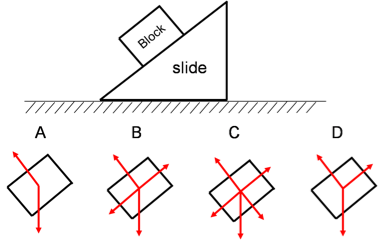
\includegraphics[scale=.4]{/Users/jgates/desktop/latex/pics/incline3.png}
%\end{floatingfigure}
 
{\bf \Large{\arabic{ProbNum}}} You're driving along the highway at constant speed.  When you increase your speed by ${7.9~\tfrac{mi}{hr}}$, the time to go one mile decreases by 13 s. 

\bigskip

What was your original speed?  

%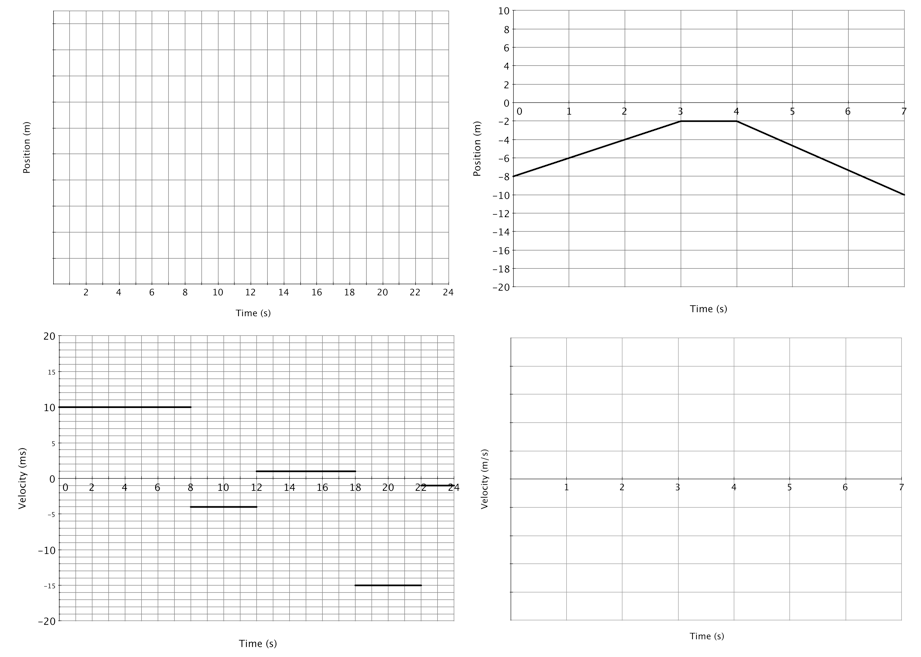
\includegraphics[scale=.57]{/Users/jgates/desktop/latex/pics/cvpmgraphs1.png}

\vfill

\newpage
